\begin{frame}
\frametitle{Contexte (2)}
\begin{center}
  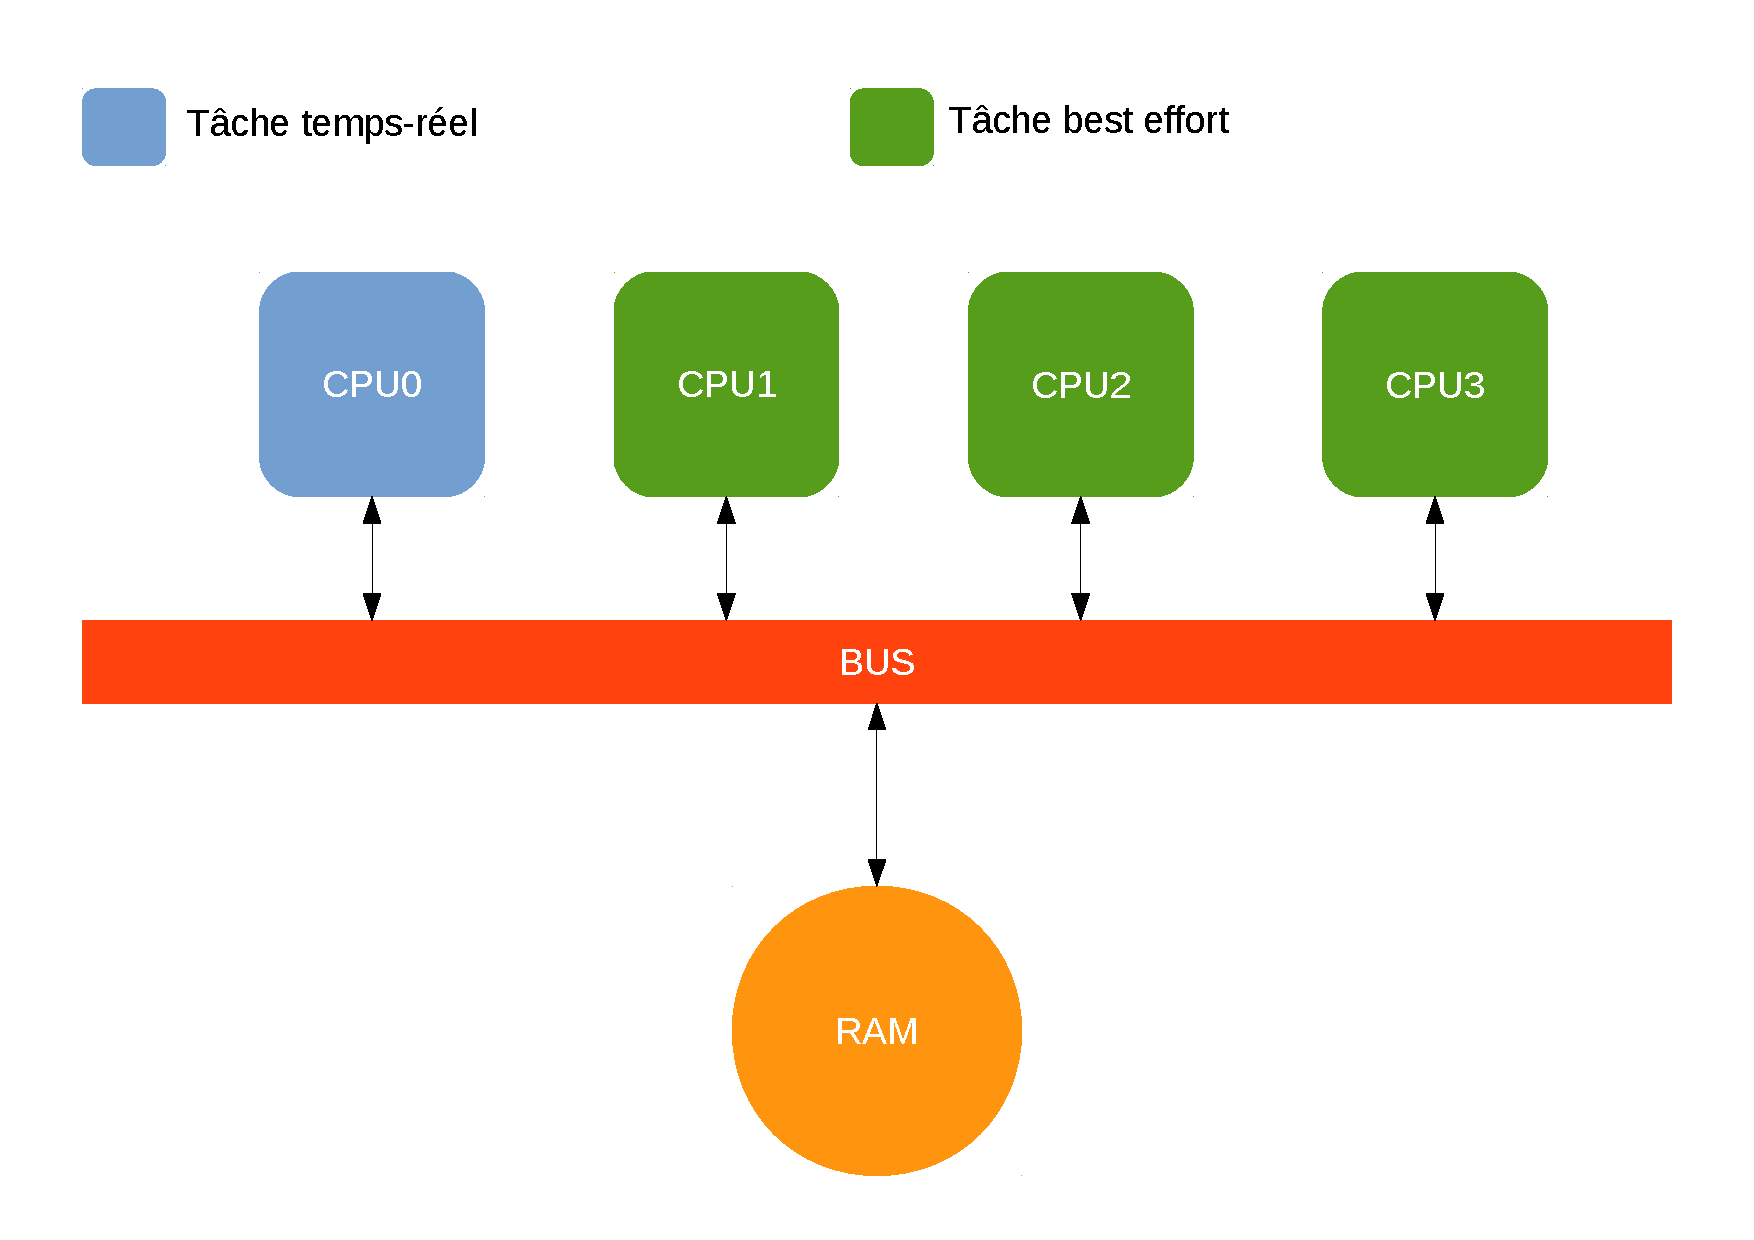
\includegraphics[scale=0.3]{include/archi.pdf}
\end{center}
\end{frame}

\begin{frame}
\frametitle{Objectifs}
\begin{itemize}
  \item Choix de l'application
    \vspace{1em}
  \item Parallélisation de l'application
    \vspace{1em}
  \item Profilage
\end{itemize}
\end{frame}

\begin{frame}
\frametitle{Choix de l'application}
\begin{itemize}
  \item Beaucoup d'accès mémoire
    \vspace{1em}
  \item Trouvable dans une voiture
\end{itemize}
\end{frame}

\begin{frame}
\frametitle{Critères de selection}
\begin{itemize}
  \item Langage
    \vspace{1em}
  \item Nombre de dépendances
    \vspace{1em}
  \item Consommation mémoire
    \vspace{1em}
  \item Parallélisable
\end{itemize}
\end{frame}


\begin{frame}
\frametitle{Open Street Routing Machine}
Inconvénients :
\begin{itemize}
\item Nombre de dépendences élevé
    \vspace{1em}
\item Consommation mémoire trop élevée
\end{itemize}
\end{frame}


\begin{frame}
\frametitle{Routino}
\begin{itemize}
\item Aucune dépendance
    \vspace{1em}
\item Peu gourmand en mémoire
    \vspace{1em}
\item ... mais pas parallèle
\end{itemize}
\end{frame}

